\documentclass[10pt,letterpaper]{article}

\usepackage[T1]{fontenc}
\usepackage[utf8]{inputenc}
\usepackage[spanish,es-noquoting]{babel}
\usepackage{lmodern}
\usepackage[margin=1.9cm,top=1.5cm,bottom=1.6cm]{geometry}
\usepackage{booktabs}
\usepackage{array}
\usepackage{xcolor}
\usepackage{graphicx}
\usepackage{fancyvrb}

\definecolor{acc}{HTML}{1F4E79}
\definecolor{gris}{HTML}{5B6672}
\definecolor{marca}{HTML}{B22222}

\setlength{\parskip}{2pt}
\setlength{\topsep}{2pt}
\setlength{\partopsep}{0pt}
\setlength{\parindent}{0pt}
\renewcommand{\arraystretch}{1.05}
\setlength{\emergencystretch}{2em}

% Secciones y pie de pagina sin paquetes externos: solo LaTeX base.
\makeatletter
\renewcommand\section{\@startsection{section}{1}{\z@}%
  {7pt \@plus 2pt \@minus 1pt}{3pt}%
  {\normalfont\normalsize\bfseries\color{acc}}}
\renewcommand\subsection{\@startsection{subsection}{2}{\z@}%
  {5pt \@plus 1pt}{2pt}%
  {\normalfont\small\bfseries\color{acc}}}
\renewcommand\@seccntformat[1]{\csname the#1\endcsname.\quad}
\renewcommand{\ps@plain}{%
  \renewcommand{\@oddhead}{}\renewcommand{\@evenhead}{}%
  \renewcommand{\@oddfoot}{\footnotesize\color{gris}%
    TI-4601 $\cdot$ Laboratorio 2 $\cdot$ One size fits all? Postgres 16 y Valkey 8
    \hfill \thepage}%
  \renewcommand{\@evenfoot}{\@oddfoot}}
\makeatother
\pagestyle{plain}

\fvset{fontsize=\footnotesize,frame=leftline,framerule=0.6pt,rulecolor=\color{gris},xleftmargin=6pt}

\begin{document}

{\LARGE\bfseries\color{acc} Laboratorio 2 --- One size fits all?}\\[2pt]
{\footnotesize\color{gris} TI-4601 Bases de Datos Avanzadas $\cdot$ Grupo 3 $\cdot$ Fabricio Mena $\cdot$ Christopher Rodriguez $\cdot$ Alisson Redondo}

\vspace{4pt}\hrule\vspace{6pt}

\section{Entorno y predicciones}

Todas las medidas salen de una sola corrida, el 17/10/2026: \texttt{cargar.py}, \texttt{analitica.py},
\texttt{escrituras.py} y \texttt{graficas.py} seguidos, desde un \texttt{resultados.jsonl} limpio.

\begin{center}\footnotesize
\begin{tabular}{@{}ll@{}}
\toprule
Máquina & Laptop AMD Ryzen 7 5700U, 4 CPU asignados a WSL 2 \\
Sistema operativo & Windows 11 Home con Ubuntu 24.04 en WSL 2, Docker Desktop 29.5.2 \\
RAM & 16 GB (9,7 GiB para WSL 2) \\
Motores & Postgres 16 y Valkey 8.1 (\texttt{-{}-appendonly no}, \texttt{-{}-maxmemory 4gb}) \\
Perfil & completo: 10\,906\,858 viajes en Postgres y 1\,000\,000 en Valkey \\
\bottomrule
\end{tabular}
\end{center}

Las predicciones están en \texttt{evidence/predicciones.md}. Las de los pasos 1 y 3 se escribieron antes
de correr cada paso. La del paso 2 se documentó después de correrlo, así que no cuenta como predicción
previa; se deja como análisis de lo esperado.

\begin{center}\footnotesize
\begin{tabular}{@{}lrr@{}}
\toprule
\textbf{Métrica} & \textbf{Predicción} & \textbf{Medido} \\
\midrule
Paso 1: carga de Postgres & $\sim$150\,000 filas/s & 165\,323 filas/s \\
Paso 1: carga de Valkey & $\sim$30\,000 filas/s & 19\,141 filas/s \\
Paso 1: bytes por fila, Postgres / Valkey & $\sim$180 / $\sim$550 & 181,5 / 549,4 \\
Paso 2: \texttt{GROUP BY} (no previa) & gana Postgres & Postgres, 81× \\
Paso 3a: lectura / update por llave & Valkey $\sim$1,5× / $\sim$20× & Valkey 1,08× / 8,8× \\
Paso 3b: \texttt{valkey\_aof\_always} vs \texttt{postgres\_commit\_por\_mensaje} & Valkey $\sim$1,3× & Postgres 2,0× \\
Paso 3b: \texttt{valkey\_pipeline} & $\sim$50\,000 msg/s & 51\,040 msg/s \\
\bottomrule
\end{tabular}
\end{center}

El espacio salió casi exacto. Fallamos en dos cosas: la carga de Valkey fue más lenta de lo previsto
(armar cada \texttt{HSET} en Python cuesta más de lo estimado) y con \texttt{appendfsync always} Valkey
quedó por debajo de Postgres, no por encima.

\section{Código de los TODO y verificaciones}

\textbf{TODO 1} (\texttt{cargar.py})
\begin{Verbatim}
    cur.execute(
        "SELECT pg_relation_size('trips'), pg_indexes_size('trips'),"
        " pg_total_relation_size('trips')"
    )
    return cur.fetchone()
\end{Verbatim}

\textbf{TODO 2} (\texttt{cargar.py})
\begin{Verbatim}
    pipe = r.pipeline(transaction=False)
    n = 0
    for n, row in enumerate(iter_rows(limit), start=1):
        pipe.hset(f"trip:{n}", mapping=dict(zip(CSV_COLUMNS, row)))
        if n % PIPELINE_BATCH == 0:
            pipe.execute()
    pipe.execute()
    return n
\end{Verbatim}

\textbf{TODO 3} (\texttt{analitica.py})
\begin{Verbatim}
    pipe = r.pipeline(transaction=False)
    for k in keys:
        pipe.hmget(k, "payment_type", "fare_amount")
    results = pipe.execute()
    for payment_type, fare_amount in results:
        if payment_type is None or fare_amount is None:
            continue
        pt = str(payment_type)
        fare = float(fare_amount)
        sums[pt] = sums.get(pt, 0.0) + fare
        counts[pt] = counts.get(pt, 0) + 1
\end{Verbatim}

\textbf{TODO 4} (\texttt{lua/feed.lua})
\begin{Verbatim}
redis.call('HINCRBY', 'agg:n', pt, 1)
redis.call('HINCRBYFLOAT', 'agg:suma', pt, fare)
if anom == '1' then
    local anomalias = redis.call('HINCRBY', 'alarma:anomalias', vendor, 1)
    if anomalias % umbral == 0 then
        redis.call('HINCRBY', 'alarma:alertas', vendor, 1)
        return 1
    end
end
return 0
\end{Verbatim}

\textbf{TODO 5} (\texttt{escrituras.py})
\begin{Verbatim}
    for i in range(0, len(msgs), batch):
        with conn.transaction(), conn.cursor() as cur:
            cur.executemany(INSERT, [m[:4] for m in msgs[i:i + batch]])
\end{Verbatim}

\textbf{Verificaciones} (\texttt{evidence/salida\_cargar.txt}, \texttt{salida\_analitica.txt} y
\texttt{salida\_escrituras.txt})
\begin{Verbatim}
  OK: TODO 1: total >= heap + índices, y ambos > 0
  OK: TODO 2: Valkey tiene 1,000,000 llaves trip:*
  OK: TODO 2: el último viaje tiene el campo fare_amount
  OK: TODO 3: el GROUP BY a mano da los mismos conteos y promedios que Postgres
  OK: postgres_commit_por_mensaje da la respuesta esperada
  OK: postgres_commit_asincrono da la respuesta esperada
  OK: postgres_lote da la respuesta esperada (TODO 5)
  OK: valkey_por_mensaje da la respuesta esperada (TODO 4)
  OK: valkey_aof_always da la respuesta esperada (TODO 4)
  OK: valkey_pipeline da la respuesta esperada (TODO 4)
\end{Verbatim}

\textbf{¿Por qué el pipeline y el lote cambian el tiempo?} Los dos atacan un costo fijo que se paga por
cada envío y no por cada fila. Sin pipeline, cada \texttt{HSET} espera su respuesta antes de mandar el
siguiente: 1\,000\,000 de viajes de ida y vuelta por la red; con lotes de 10\,000 son 100. En el feed,
\texttt{valkey\_pipeline} pasa de 2\,336 a 51\,040 msg/s (22×) con exactamente el mismo trabajo en el
servidor. El lote de Postgres (TODO 5) junta 1\,000 mensajes por transacción: el trigger corre igual por
cada fila, pero el WAL se espera en disco 10 veces y no 10\,000, y \texttt{executemany} manda las filas
sin esperar la respuesta de cada \texttt{INSERT}. Pasa de 486 a 29\,792 msg/s (61×). \texttt{COPY}
sigue la misma idea en la carga: un solo flujo de bytes y un solo commit, sin un \texttt{INSERT} por fila.

\section{Resultados}

\begin{center}
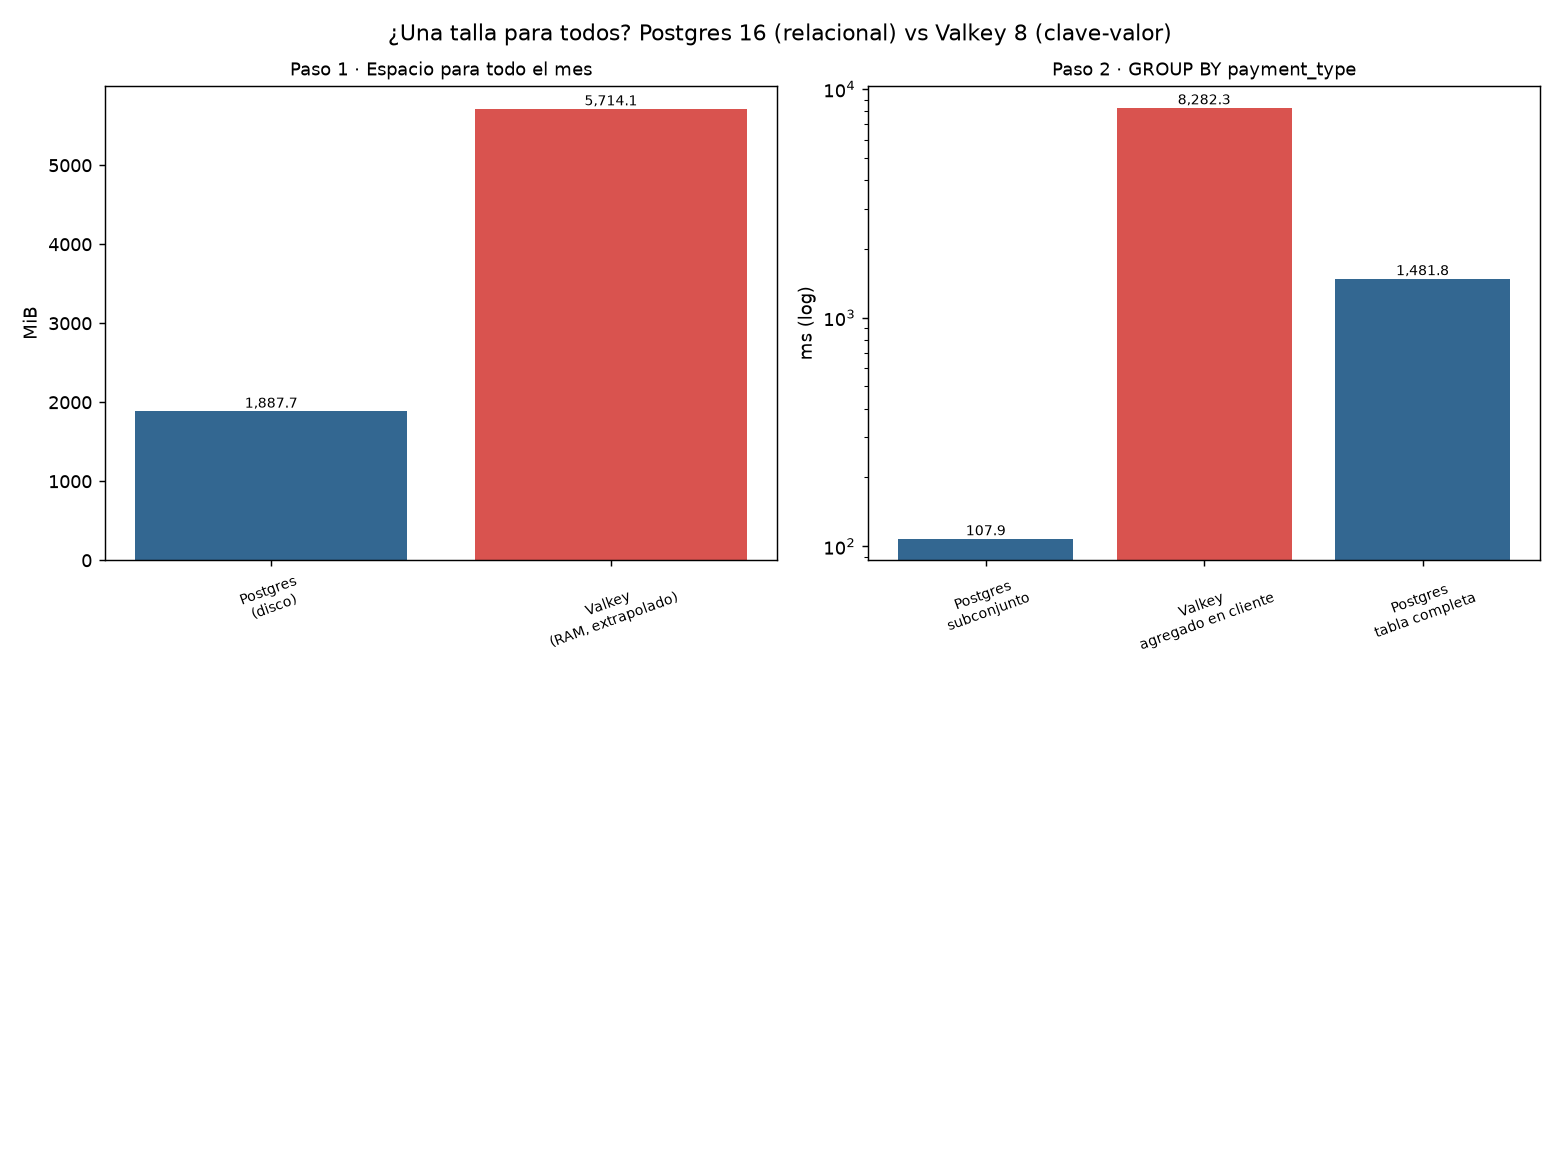
\includegraphics[width=0.8\textwidth]{evidence/graficas.png}
\end{center}

\subsection{Paso 1: carga y espacio}

\begin{center}\footnotesize
\begin{tabular}{@{}lrr@{}}
\toprule
& \textbf{Postgres} & \textbf{Valkey} \\
\midrule
Filas cargadas & 10\,906\,858 & 1\,000\,000 \\
Tiempo & 66,0 s \texttt{COPY} + 10,0 s índice PK & 52,2 s \\
Filas por segundo & 165\,323 & 19\,141 \\
Espacio medido & 1\,653,6 MiB tabla + 233,7 MiB índice & 523,9 MiB de RAM \\
Bytes por fila & 181,5 & 549,4 \\
Mes completo & 1\,887,7 MiB de disco & 5\,714,2 MiB de RAM (extrapolado) \\
\bottomrule
\end{tabular}
\end{center}

\textbf{¿Qué tienen en común los dos métodos de carga?} Los dos evitan mandar un comando por fila y
esperar su respuesta. \texttt{COPY} manda el CSV como un solo flujo de bytes en una transacción y el
servidor lo parsea; el pipeline junta 10\,000 \texttt{HSET} y los manda juntos. Aun así Valkey cargó
8,6 veces más lento: con \texttt{COPY} Python solo pasa líneas de texto, y con Valkey tiene que armar
cada \texttt{HSET} con 19 pares campo-valor.

\textbf{¿Qué pasa si el TODO 1 falla después del \texttt{COPY}?} La conexión usa autocommit, así que
el \texttt{COPY}, la llave primaria y el \texttt{VACUUM} ya están confirmados. La tabla queda cargada,
pero el script se detiene: no se registran las medidas de disco ni se carga Valkey. Al volver a correr,
\texttt{pg\_trips.sql} hace \texttt{DROP TABLE} y la carga se repite completa (unos 76~s).

\textbf{Bytes por fila y espacio total.} Valkey usa 549,4 B por viaje y Postgres 181,5 B (159 de la
tabla y 22 del índice), 3,0 veces menos. Postgres guarda cada valor con su tipo y los nombres de columna
una sola vez, en el esquema; Valkey guarda todo como texto y repite los 19 nombres de campo en cada
viaje. El mes completo serían 5\,714 MiB de RAM contra 1\,888 MiB de disco, y no cabe en los 4 GB del
Valkey del curso.

\textbf{¿Qué motor podría guardar un año entero en una laptop?} Postgres. Un año son unos 131 M de
viajes: unos 22 GiB de disco en Postgres contra unos 67 GiB de RAM en Valkey. Esta laptop tiene 16 GB
de RAM.

\subsection{Paso 2: consulta de almacén}

\begin{center}\footnotesize
\begin{tabular}{@{}lrr@{}}
\toprule
& \textbf{Postgres} & \textbf{Valkey} \\
\midrule
\texttt{GROUP BY} sobre el mismo millón de viajes (mediana) & 170,8 ms & 13\,882,7 ms \\
\texttt{GROUP BY} sobre la tabla completa (mediana) & 1\,064,9 ms & --- \\
Pregunta nueva: propina promedio por hora & 1\,329,4 ms & --- \\
\bottomrule
\end{tabular}
\end{center}

Sobre las mismas filas Postgres fue 81 veces más rápido. Valkey no tiene \texttt{GROUP BY}: el cliente
recorrió las llaves con \texttt{SCAN}, trajo dos campos de cada viaje con \texttt{HMGET} y sumó en
Python (el TODO 3 es el \texttt{HashAggregate} hecho a mano). La pregunta no anticipada se responde en
Postgres con un \texttt{SELECT} nuevo sobre los mismos datos; en Valkey habría que escribir otro
recorrido en el cliente.

\subsection{Paso 3: escrituras y feed}

\begin{center}\footnotesize
\begin{tabular}{@{}lrrl@{}}
\toprule
\textbf{3a, mediana de 2\,000} & \textbf{Postgres} & \textbf{Valkey} & \textbf{Gana} \\
\midrule
Lectura por llave & 0,341 ms & 0,316 ms & Valkey, 1,08× (casi empate) \\
Update por llave & 2,280 ms & 0,258 ms & Valkey, 8,8× \\
\bottomrule
\end{tabular}
\end{center}

La lectura es casi empate: en el servidor los dos hacen muy poco y lo que se mide es la red y el cliente.
En el update, cada \texttt{UPDATE} de Postgres con autocommit espera a que el WAL llegue a disco con
\texttt{fsync}; esos 1,9 ms de más son el precio de la D de ACID. Valkey cambia el valor en RAM y responde.

\begin{center}\footnotesize
\begin{tabular}{@{}lrrl@{}}
\toprule
\textbf{3b, 10\,000 mensajes} & \textbf{msg/s} & \textbf{ms/msg} & \textbf{¿Espera al disco por mensaje?} \\
\midrule
\texttt{postgres\_commit\_por\_mensaje} & 486 & 2,059 & Sí (WAL) \\
\texttt{postgres\_commit\_asincrono} & 1\,847 & 0,541 & No \\
\texttt{postgres\_lote} & 29\,792 & 0,034 & Una vez por lote \\
\texttt{valkey\_por\_mensaje} & 2\,336 & 0,428 & No \\
\texttt{valkey\_aof\_always} & 240 & 4,167 & Sí (AOF) \\
\texttt{valkey\_pipeline} & 51\,040 & 0,020 & No \\
\bottomrule
\end{tabular}
\end{center}

Las seis variantes dan 7 alertas y los mismos conteos. Postgres procesa \emph{outbound}: guarda el mensaje
en \texttt{feed\_trip} (versión de fila, heap y WAL) y después el trigger hace dos
\texttt{INSERT … ON CONFLICT}. Valkey procesa \emph{inbound}: el mensaje no se guarda, pasa por
\texttt{feed.lua} dentro del servidor y solo quedan cuatro contadores. Con el Count100 exacto del paper
(50\,000 mensajes, umbral 100) las conclusiones no cambian (\texttt{evidence/paso3.md}).

\subsection{Tabla de medidas (\texttt{evidence/tabla.md})}

\begin{center}\scriptsize
\begin{tabular}{@{}lllrl@{}}
\toprule
\textbf{Paso} & \textbf{Motor} & \textbf{Métrica} & \textbf{Valor} & \textbf{Unidad} \\
\midrule
1-carga & postgres & bytes\_por\_fila & 181.482 & B/fila \\
1-carga & postgres & disco\_indices & 233.656 & MiB \\
1-carga & postgres & disco\_tabla & 1,653.562 & MiB \\
1-carga & postgres & disco\_total & 1,887.703 & MiB \\
1-carga & postgres & filas & 10,906,858 & filas \\
1-carga & postgres & filas\_por\_s & 165,323.443 & filas/s \\
1-carga & postgres & tiempo\_copy & 65.973 & s \\
1-carga & postgres & tiempo\_indice\_pk & 9.982 & s \\
1-carga & valkey & bytes\_por\_fila & 549.356 & B/fila \\
1-carga & valkey & filas & 1,000,000 & filas \\
1-carga & valkey & filas\_por\_s & 19,140.676 & filas/s \\
1-carga & valkey & ram\_extrapolada\_total & 5,714.171 & MiB \\
1-carga & valkey & ram\_usada & 523.906 & MiB \\
1-carga & valkey & tiempo\_carga & 52.245 & s \\
2-olap & postgres & explain\_execution\_time & 1,445.133 & ms \\
2-olap & postgres & mediana\_completa & 1,064.854 & ms \\
2-olap & postgres & mediana\_subconjunto & 170.836 & ms \\
2-olap & postgres & pregunta\_nueva & 1,329.447 & ms \\
2-olap & valkey & agregado\_en\_cliente & 13,882.670 & ms \\
3a-puntual & postgres & lectura\_por\_llave\_p50 & 0.341 & ms \\
3a-puntual & postgres & update\_por\_llave\_p50 & 2.280 & ms \\
3a-puntual & valkey & lectura\_por\_llave\_p50 & 0.316 & ms \\
3a-puntual & valkey & update\_por\_llave\_p50 & 0.258 & ms \\
3b-feed & postgres\_commit\_asincrono & leer\_respuesta & 0.566 & ms \\
3b-feed & postgres\_commit\_asincrono & mensajes\_por\_s & 1,847.409 & msg/s \\
3b-feed & postgres\_commit\_por\_mensaje & leer\_respuesta & 0.921 & ms \\
3b-feed & postgres\_commit\_por\_mensaje & mensajes\_por\_s & 485.707 & msg/s \\
3b-feed & postgres\_lote & leer\_respuesta & 1.166 & ms \\
3b-feed & postgres\_lote & mensajes\_por\_s & 29,792.325 & msg/s \\
3b-feed & valkey\_aof\_always & leer\_respuesta & 0.780 & ms \\
3b-feed & valkey\_aof\_always & mensajes\_por\_s & 239.968 & msg/s \\
3b-feed & valkey\_pipeline & leer\_respuesta & 0.895 & ms \\
3b-feed & valkey\_pipeline & mensajes\_por\_s & 51,040.470 & msg/s \\
3b-feed & valkey\_por\_mensaje & leer\_respuesta & 0.664 & ms \\
3b-feed & valkey\_por\_mensaje & mensajes\_por\_s & 2,336.417 & msg/s \\
\bottomrule
\end{tabular}
\end{center}

\section{Plan de Postgres (\texttt{evidence/plan\_olap\_postgres.txt})}

\begin{Verbatim}[fontsize=\fontsize{6}{7.2}\selectfont,commandchars=\\\{\}]
Finalize GroupAggregate  (cost=292188.85..292189.91 rows=4 width=42) (actual time=1436.467..1443.935 rows=5 loops=1)
  Group Key: payment_type
  Buffers: shared hit=14 read=211656
  ->  Gather Merge  (cost=292188.85..292189.78 rows=8 width=42) (actual time=1436.392..1443.842 rows=13 loops=1)
        Workers Planned: 2
        Workers Launched: 2
        Buffers: shared hit=14 read=211656
        ->  Sort  (cost=291188.82..291188.83 rows=4 width=42) (actual time=1420.062..1420.063 rows=4 loops=3)
              Sort Key: payment_type
              Sort Method: quicksort  Memory: 25kB
              Buffers: shared hit=14 read=211656
              Worker 0:  Sort Method: quicksort  Memory: 25kB
              Worker 1:  Sort Method: quicksort  Memory: 25kB
\textcolor{marca}{\textbf{              ->  Partial HashAggregate  (cost=291188.73..291188.78 rows=4 width=42) (actual time=1420.039..1420.042 rows=4 loops=3)  <== nodo dominante}}
                    Group Key: payment_type
                    Batches: 1  Memory Usage: 24kB
                    Buffers: shared read=211656
                    Worker 0:  Batches: 1  Memory Usage: 24kB
                    Worker 1:  Batches: 1  Memory Usage: 24kB
\textcolor{marca}{\textbf{                    ->  Parallel Seq Scan on trips  (cost=0.00..257103.27 rows=4544728 width=7) (actual time=0.046..459.170 rows=3635619 loops=3)}}
\textcolor{marca}{\textbf{                          Buffers: shared read=211656  <== 211 656 x 8 KiB = 1 653,6 MiB = disco_tabla}}
Planning:
  Buffers: shared hit=39 read=7
Planning Time: 1.424 ms
JIT:
  Functions: 21
  Options: Inlining false, Optimization false, Expressions true, Deforming true
  Timing: Generation 2.210 ms, Inlining 0.000 ms, Optimization 1.800 ms, Emission 22.603 ms, Total 26.613 ms
Execution Time: 1445.133 ms
\end{Verbatim}

Leído de abajo hacia arriba:

\textbf{Parallel Seq Scan.} Dos workers más el proceso principal (\texttt{loops=3}), unas 3\,635\,619
filas cada uno, 10,9 M en total, en 459 ms. Leyó 211\,656 páginas de 8 KiB:
$211\,656 \times 8 / 1024 = 1\,653{,}6$ MiB, exactamente el \texttt{disco\_tabla} del paso 1. Postgres
leyó la tabla entera para responder.

\textbf{Agregación en dos fases.} Cada worker calcula su \texttt{Partial HashAggregate} por
\texttt{payment\_type}; \texttt{Gather Merge} junta los resultados parciales y
\texttt{Finalize GroupAggregate} produce los 5 grupos finales.

\textbf{Nodo dominante.} El \texttt{Partial HashAggregate} con su escaneo toma 1\,420 de los 1\,445 ms
(98~\%): 459 ms de escaneo y el resto en agrupar y promediar 10,9 M filas. Todo el costo depende de cuántas
filas y páginas se recorren, y aquí está el row-store: la consulta usa dos columnas (el escaneo entrega
\texttt{width=7} bytes por fila), pero cada página trae las 20 columnas, unos 159 B por fila. Para usar
dos columnas se leyeron 1\,653,6 MiB. Eso es lo que un column-store evita.

\clearpage
\section{Respuesta: ¿por qué «One Size Fits All» es una idea desfasada?}

Stonebraker y Çetintemel parten de que los motores comerciales se diseñaron para el procesamiento de
datos de negocio (OLTP) y que los fabricantes mantuvieron una sola línea de código para todo
(sección 1). Su tesis es que esa estrategia ya falló en los almacenes de datos (sección 2) y que falla
todavía más en el procesamiento de flujos (secciones 3 y 4), porque cada mercado necesita una
arquitectura distinta (sección 7). El laboratorio repite la idea en pequeño: los mismos viajes de taxi
en un motor relacional y en uno clave-valor, con tres cargas de trabajo distintas.

\textbf{1. Ningún motor gana todas las cargas de trabajo.} En el paso 1 gana Postgres: cargó el mes
completo a 165\,323 filas/s, 8,6 veces más rápido que Valkey (19\,141 filas/s), y cada viaje ocupa 181 B
en disco contra 549 B en RAM, 3,0 veces menos. En el paso 2 también gana Postgres, por 81× (punto 2). En
el paso 3 gana Valkey: el update por llave le toma 0,26 ms contra 2,28 ms de Postgres (8,8×), y en el
feed \texttt{valkey\_pipeline} procesa 51\,040 mensajes/s, 1,7 veces más que la mejor variante de
Postgres (\texttt{postgres\_lote}, 29\,792) y 105 veces más que un commit por mensaje (486). La lectura
por llave queda casi empatada (0,32 contra 0,34 ms).

Los números también muestran las limitantes de Valkey. Todo tiene que caber en RAM: el mes completo
necesitaría 5\,714 MiB, que no caben en los 4 GB que tiene asignados, y un año serían unos 67 GiB contra
22 GiB de disco en Postgres. No tiene tipos ni esquema, así que guarda todo como texto y repite los 19
nombres de campo en cada viaje. No tiene \texttt{GROUP BY}. Y su ventaja en el paso 3 depende de no
escribir a disco: con \texttt{appendfsync always} baja a 240 mensajes/s. Cada motor gana donde su diseño
calza con la carga.

\textbf{2. Que Valkey pierda el \texttt{GROUP BY} no refuta el argumento del data warehouse.} En el paso
2 Postgres respondió el \texttt{GROUP BY payment\_type} sobre el mismo millón de viajes en 171 ms y Valkey
en 13\,883 ms. Podría parecer que esto contradice al paper, que dice que un row-store no es lo mejor para
un almacén. No es así, por dos razones.

Primero, el experimento no enfrenta un row-store contra un column-store, sino un motor que tiene la
primitiva de agregación contra uno que no la tiene. Valkey solo sabe responder «dame el valor de esta
llave»: el cliente tuvo que recorrer las llaves con \texttt{SCAN}, traer dos campos de cada viaje con
\texttt{HMGET} y sumar en Python. Postgres agregó dentro del motor, en paralelo y en dos fases
(\texttt{Partial HashAggregate} y \texttt{Finalize GroupAggregate}). Es el argumento de la sección 4.2:
sin la primitiva correcta en el motor se pierde, sin importar cómo se guarden los datos.

Segundo, el plan de Postgres muestra justo el costo que el paper le atribuye al row-store. El escaneo y
la agregación parcial toman el 98~\% del tiempo, y el escaneo leyó 211\,656 páginas, 1\,653,6 MiB: la
tabla entera, con sus 20 columnas, para usar dos. Un column-store leería solo esas dos columnas, que es
la ventaja que describe la sección 5.1 para consultas que agregan pocos atributos de muchas filas. Lo que
sí confirma el paso 2 es la sección 2: Postgres respondió en 1\,329 ms una pregunta que nadie previó (la
propina promedio por hora), mientras que Valkey solo tiene lo que se guardó para responder por llave.

\textbf{3. La brecha no es solo el overhead de \texttt{fsync()}.} En el paper, StreamBase procesó
160\,000 mensajes por segundo y el RDBMS 900 (sección 4). La explicación fácil es que el RDBMS escribe a
disco y el motor de flujos no. Con los dos pares del paso 3b se puede separar qué parte es durabilidad y
qué parte es modelo.

En el par con durabilidad (\texttt{valkey\_aof\_always} contra \texttt{postgres\_commit\_por\_mensaje})
los dos esperan al disco en cada mensaje, y gana Postgres: 486 contra 240 msg/s (2,0×). El
\texttt{fsync} se come el 74~\% del tiempo de Postgres y el 90~\% del de Valkey. Cuando los dos
garantizan la D en cada mensaje, gana la bitácora mejor optimizada, no el modelo en memoria.

En el par sin durabilidad (\texttt{valkey\_por\_mensaje} contra \texttt{postgres\_commit\_asincrono})
ninguno espera al disco, y gana Valkey: 2\,336 contra 1\,847 msg/s (1,26×). Esa diferencia ya no es
\texttt{fsync}, es el modelo. Postgres procesa outbound: guarda el mensaje en \texttt{feed\_trip} y luego
el trigger hace dos upserts. Valkey procesa inbound: el mensaje pasa por un script Lua dentro del
servidor y solo quedan los contadores (secciones 4.1 y 4.3). Con la red repartida en lotes de 1\,000, la
ventaja del modelo sube a 1,7× (\texttt{valkey\_pipeline} 51\,040 contra \texttt{postgres\_lote}
29\,792).

Así, de la brecha de 105× entre \texttt{postgres\_commit\_por\_mensaje} y \texttt{valkey\_pipeline},
quitar el \texttt{fsync} explica solo 3,8×; agrupar los mensajes en lotes explica 16×, y el modelo deja
1,7× que no desaparece. El paper también explica por qué StreamBase no necesita ese \texttt{fsync}: logra
alta disponibilidad con réplicas en vez de una bitácora en disco (sección 4.4) y no necesita
transacciones ACID completas (sección 4.5).

\textbf{Conclusión.} Los tres pasos muestran lo mismo que el paper: el diseño que gana una carga pierde
otra. El row-store con transacciones guarda, carga y agrega mejor; el motor en memoria que procesa el
mensaje adentro gana las operaciones por llave y el feed, pero solo mientras no tenga que guardar nada.
Para hacerlo todo bien, un solo producto tendría que llevar varias arquitecturas por dentro, que es justo
lo que el paper llama el fin de «one size fits all» (sección 7).

\end{document}
